\section{Evaluation}

\subsection{Inuition}

\subsection{Methodology}

We perform two evaluations.
The first informal study examines the user experience of developing one-off \glspl{name}, general-purpose \glspl{name}, and interactions for accessing additional information through \glspl{name} as a tutorial reader.
The second, formal in-lab study verifies hypotheses including:
\noindent
\begin{enumerate}%[label=\textbf{H\arabic*.}, ref=H\arabic*, leftmargin=*]
\item Users find \glspl{name} generate helpful, relevant explanations.
\item Users without familiarity with the grammars described by \glspl{name} gain better conceptual understanding.
\end{enumerate}

\subsection{Results}

User perceptions of explanation relevance and helpfulness are shown in Figure~\ref{fig:user_study_bar}.
We also show the change in conceptual understanding of users of topics explained by \glspl{name} in Figure~\ref{fig:concept_bar}.

\begin{figure}
\centering{
    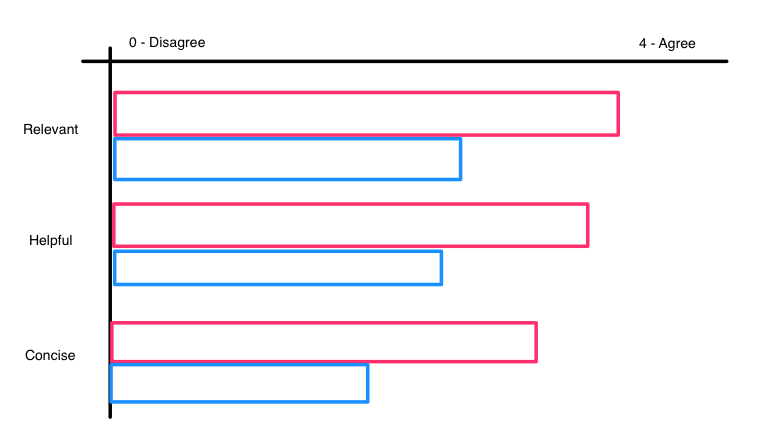
\includegraphics[width=.4\textwidth]{figures/user_study_bar}
}
\caption{Users found our explanations concise, relevant, and helpful.}
\label{fig:user_study_bar}
\end{figure}
